%! Author = raphael
%! Date = 12/10/24

% Preamble
\documentclass[11pt]{article}

\usepackage[french]{babel}

\usepackage[style=numeric, sorting=none, backend=biber]{biblatex}
\addbibresource{samReader.bib}

% Packages
\usepackage{float}
\usepackage{makecell} % Pour permettre les cellules sur plusieurs lignes
\usepackage{amsmath}
\usepackage[bottom=25mm, top=25mm]{geometry}
\usepackage{graphicx}
\usepackage{titlesec}
\usepackage{booktabs} % Pour des tableaux plus esthétiques


\usepackage[hidelinks]{hyperref}

\usepackage{caption}
\captionsetup[table]{name=Tableau}
\captionsetup[figure]{name=Figure}

% Document
\begin{document}

\begin{titlepage}
    \begin{center}
        % Logos
        
\includegraphics[width=0.4\textwidth]{UM} \hfill{} % Replace with your first logo
        
\includegraphics[width=0.4\textwidth]{FDS} % Replace with your third logo

        \vspace{3cm}

        % Title with bars
        \hrulefill\\[0.4cm]
        {\Huge \textbf{Projet Bioinformatique : samReader}}\\[0.4cm]
        \hrulefill

        \vspace{1.5cm}

        \large{\textbf{Raphaël Ribes}}\\[0.5cm]

        \vfill

        % Horizontal image near the bottom
        \url{https://github.com/RaphaelRibes/samReader}
        \href{https://github.com/RaphaelRibes/samReader}{%
            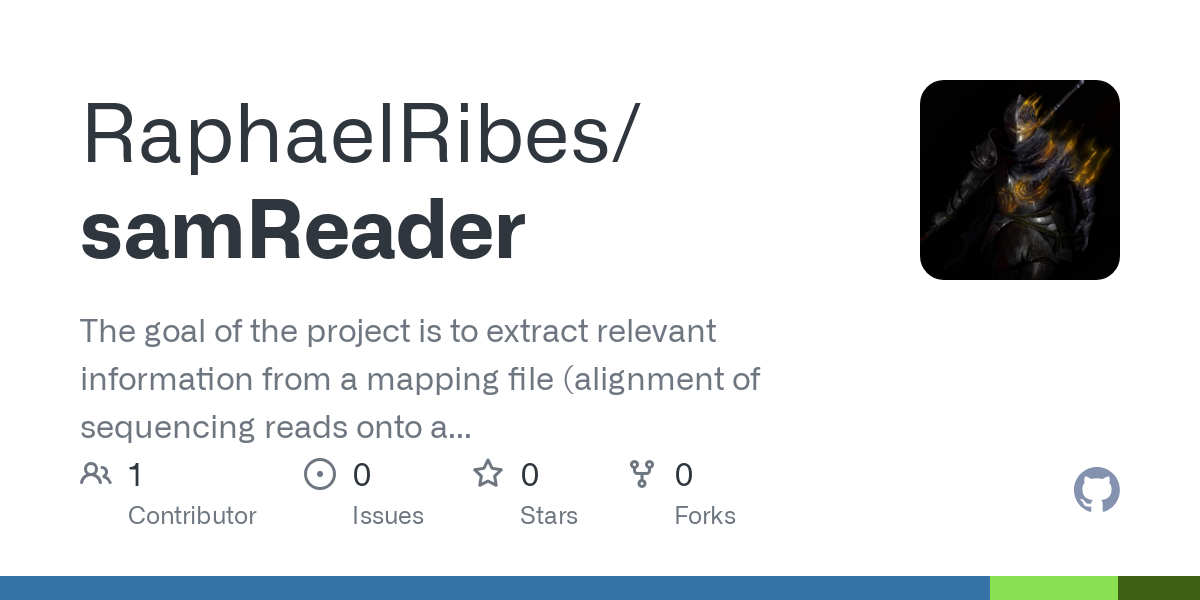
\includegraphics[width=0.8\textwidth]{samReader} % Replace with your horizontal image
        }
    \end{center}
\end{titlepage}

\section{Introduction}\label{sec:introduction}
Depuis l'émergence des technologies de séquençage de nouvelle génération (NGS), le volume et la complexité des données de séquences ADN ont augmenté de manière exponentielle.
Ces technologies, bien que révolutionnaires, génèrent des courts fragments de séquences ADN, appelés reads, qu'il est nécessaire d'aligner sur une séquence de référence pour les analyser efficacement.
Afin de standardiser et de faciliter le stockage et la manipulation de ces données d'alignement, le format SAM (Sequence Alignment/Map) a été introduit par Heng Li et Bob Handsaker \textit{et al.} en 2009\cite{li_sequence_2009}.

\noindent Le format SAM offre une solution simple et flexible pour organiser les résultats d'alignement grâce à un fichier tabulé structuré, comprenant une section d'en-tête et une section de données d'alignement.
Ce format, ainsi que son grand frère le format BAM, sont devenus indispensable pour des applications variées en biologie plus particulièrement en sciences omique.
\\\\
Ce Programme vise à lire, analyser et extraire les informations essentielles des fichiers SAM\@.
Le but est de faciliter l'interprétation des alignements, leur profondeur et leur qualité.
Cet outil permet une analyse des données issues des technologies de NGS plus simple et compréhensible pour les chercheurs.


\section{Présentation du format SAM}\label{sec:presentation-du-format-sam}
\input{présentation-du-format-sam}

\section{Exemple d'application}\label{sec:exemple-d'application}


\section{Description du programme}\label{sec:description-du-programme}

Le programme commence en premier avec le script \texttt{samReader.sh}, qui avant de lancer le programme, réalise plusieurs étapes préliminaires :
\begin{itemize}
\item La lecture et validation des options et arguments en ligne de commande.
\item La vérification de la sélection d'une version de SAM.
\item Si l’option --trusted est activée, le fichier est directement traité sans validation supplémentaire.
\item La vérification du fichier d’entrée (existence, non-vide, conformité au format SAM).
\end{itemize}

\noindent Ensuite, le script \texttt{main.py} est exécuté.
Ce dernier va itérer sur chaque ligne du fichier SAM, et vérifier (si l’option --trusted est désactivée) la conformité de chaque ligne au format SAM.
Il va aussi lors de cette étape, convertir les flags en binaire et récupérer la position du dernier read ainsi que son CIGAR.

Le programme va ensuite créer un répertoire \texttt{temp} dans lequel il va stocker les fichiers temporaires nécessaires à la génération des rapports.


\noindent Si tout est correct, exécution du script Python main.py avec les arguments adaptés.


\section{Discussion}\label{sec:discussion}

\texttt{samReader} présente des points forts significatifs, notamment la capacité à générer des rapports détaillés et personnalisés.
Ces rapports, produits sous forme de fichiers PDF, synthétisent les analyses de manière claire et exhaustive.
L’analyse approfondie des mutations fournit des statistiques générales sur les anomalies présentes dans les reads.
De plus, la segmentation des données par chromosomes améliore la lisibilité en regroupant les reads alignés, partiellement alignés et non alignés dans des répertoires distincts.
L’évaluation de la profondeur de couverture et la représentation de l’évolution de la qualité d’alignement sont aussi des fonctionnalités précieuses pour les chercheurs.


Cependant, plusieurs limitations freinent l’efficacité du programme.
La lenteur de son exécution constitue un obstacle majeur, en grande partie en raison de la génération des rapports et des graphiques, particulièrement via \LaTeX.
La représentation base par base de la qualité et de la profondeur de mappage est également problématique, limitant la précision des analyses.
Par ailleurs, le traitement des données de qualité de mappage n’est pas optimal : lorsque deux reads se superposent, l’information précédente est écrasée, ce qui peut entraîner une perte de données essentielles.


Pour améliorer ces aspects, des pistes d’optimisation sont envisageables.
La vitesse d’exécution pourrait être augmentée par une relecture plus efficace des reads et une \\ implémentation dynamique des graphiques.
Une meilleure gestion des données MAPQ est également recommandée, en stockant séparément les valeurs pour chaque base et en calculant ultérieurement une moyenne ou une médiane.
L'implémentation des différentes versions de SAM reste encore perfectible.
Bien que les idées soient présentes, leur réalisation nécessite des ajustements et des améliorations pour atteindre une architecture satisfaisante.
Ces ajustements permettraient d’accroître la précision et la rapidité du programme tout en conservant sa flexibilité.

\addcontentsline{toc}{section}{References}
\printbibliography

\end{document}